\documentclass[10pt,a4paper]{article}
\usepackage[latin1]{inputenc}
\usepackage[margin=1in]{geometry}
\usepackage{amsmath}
\usepackage{amsfonts}
\usepackage{amssymb}
\usepackage{graphicx}
\begin{document}
	
\section{Quick Disconnect}

\begin{figure}[h!]
	\centering
	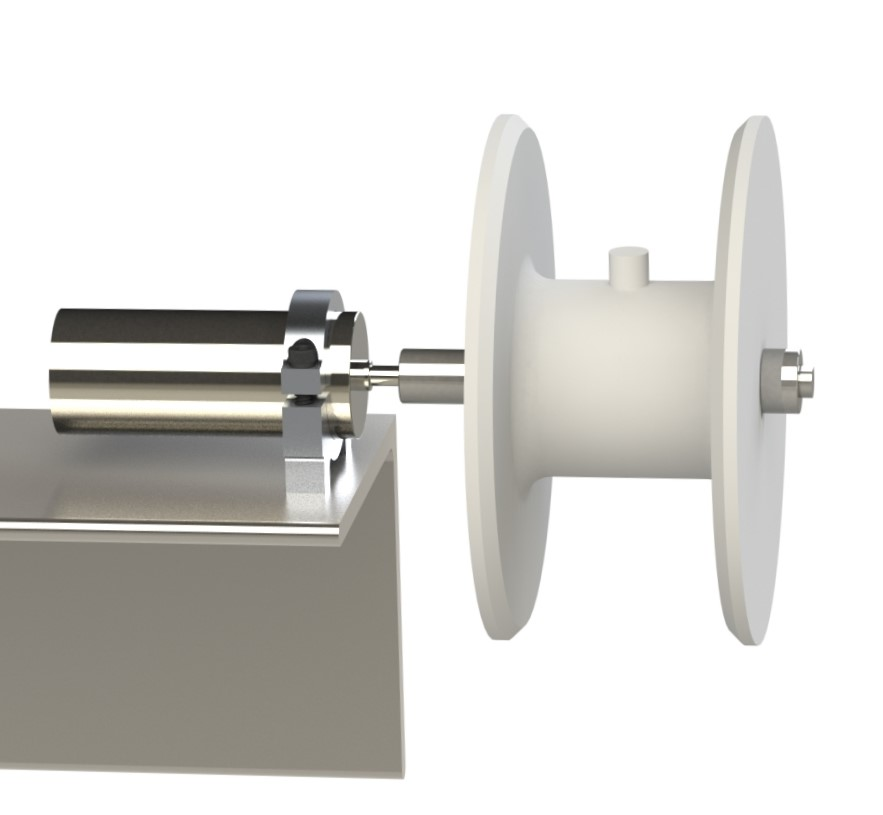
\includegraphics[width=0.3\textwidth]{./figs/qd_main.jpg}
	\caption{Quick Disconnect Pulley}
	\label{fig:qd_main}
\end{figure}


\begin{table}[h!]
		\centering
		\begin{tabular}{l l }
			Disconnecting Force & 4 lbs \\
			Required Motor Torque & 3 lb-in \\
			Motor Max Torque & 167.38 lb-in\\
			Motor Current (No Load-Stall) & .12 - 3.9 A\\
			Assembly Weight & 2.87 lbs \\
			Motor voltage & 12v\\
			Power requirements & 18Ah 12v SLA battery\\
			Motor & RobotZone 19RPM Econ Gear Motor\\
			
			
		\end{tabular}
		\caption{Subsystem Specifications}
		\label{tab:example}
\end{table} 
\subsection{Intro}
The quick disconnect system allows for the remote disconnection of the engine's nitrous fill and vent lines. The system must be remotely triggered via launch box commands and must reliably remove the fluid lines during a test or launch. 
\subsection{Design}
\subsubsection{An overview of the Old System}
	The old quick disconnect system utilizes a compressed air system with pneumatic pistons. A small compressed air tank is filled from a compressor before any test or launch and is then hooked up to the pneumatic pistons via hoses. A solenoid is connected between the hose and air tank so that the tank can be remotely opened and the lines pressurized. When the lines pressurize the pistons retract and pull the male end of the fuel line connection away. The entire assembly is clamped to the door of the test cell or launch tower as needed. This system has had numerous issues which have led to the desire for a completely new configuration. The air tank used tends to leak preventing it from being filled in advance of tests and when using two pneumatic pistons, the single air tank does not provide enough force to disconnect the lines. This second problem could be fixed using an additional air tank and solenoid, however this increases the complexity of an already over-complex system. A more simple, robust design is required.

\subsubsection{An Overview of the New System}
	The new system completely does away with compressed air and pneumatics due to the increased chance of failure. Instead the configuration uses two 12 volt motors hooked up in series with a 12v 18Ah Sealed Lead Acid Battery. This connection is routed through a relay in the launch box which can be actuated remotely to turn on and off the motors. The output shaft of the motor is connected to a set screw shaft coupler which allows a quarter inch D-shaft to be attached to the motors 4mm shaft. The quarter inch shaft runs through a 3D printed pulley and is capped on the other end with a set screw shaft collar to prevent the pulley from sliding. The 3D printed pulley has a hole with the dimensions of the D-shaft rather than just a circular shaft. This is to allow torque to be effectively transferred from the motor to the pulley without any slippage. The pulley itself has a peg to which the male quick disconnect wire is tied to and then wound around the cylinder of the pulley. When the motors are activated the pulley spools and pulls the line to disconnect the fill and vent lines. This assembly is clamped to the test cell door during tests (see figure \ref{fig:qd_setup})and bolted to a cross beam when used on the launch tower.

\subsubsection{Final Specifications} 

\begin{figure}[h!]
	\centering
	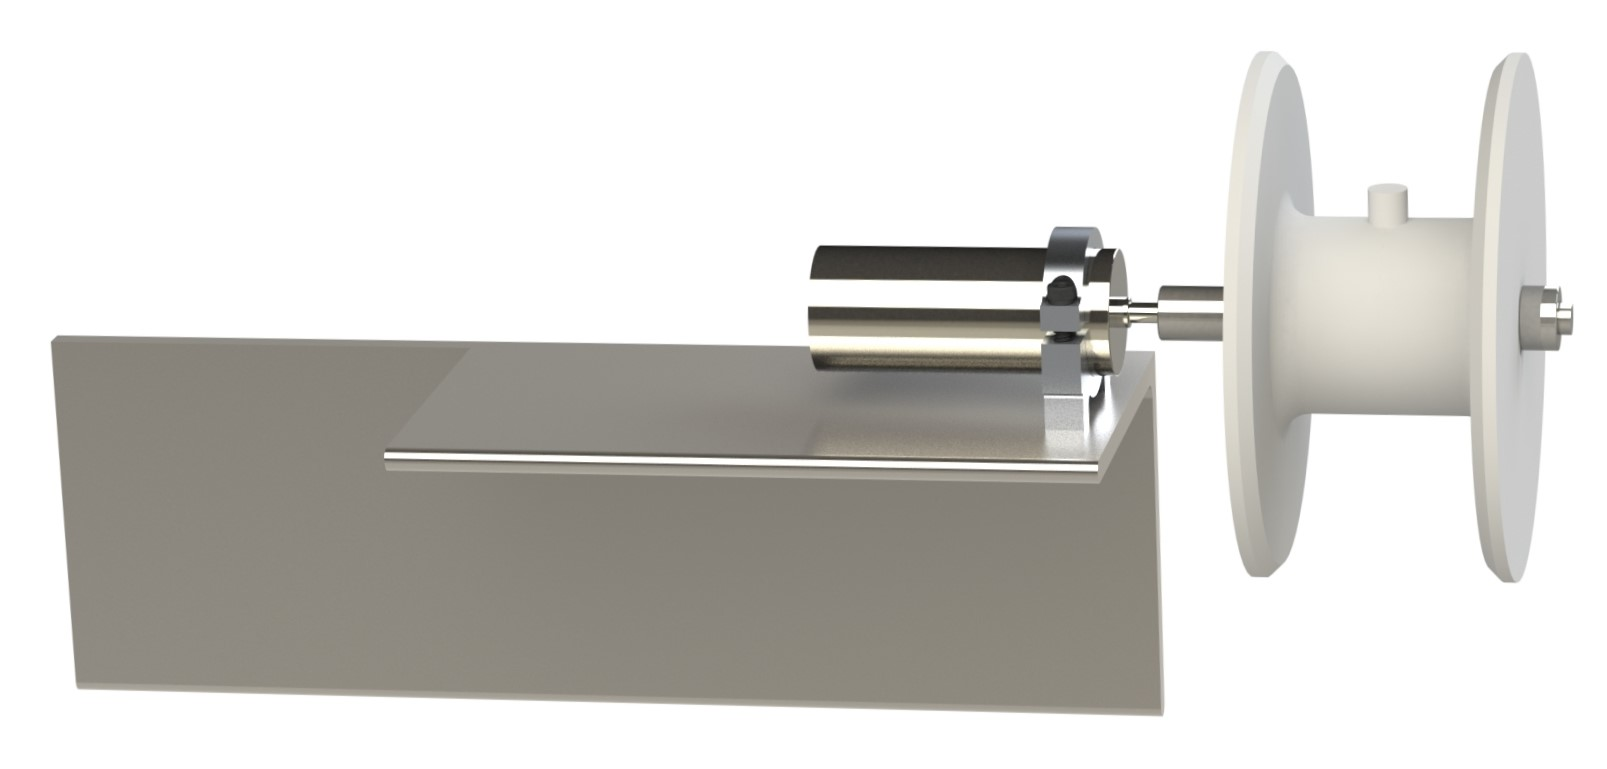
\includegraphics[width=0.9\textwidth]{./figs/qd_render.jpg}
	\caption{Solidworks Render}
	\label{fig:qd_render}
\end{figure}
	 
\begin{figure}[h!]
	\centering
	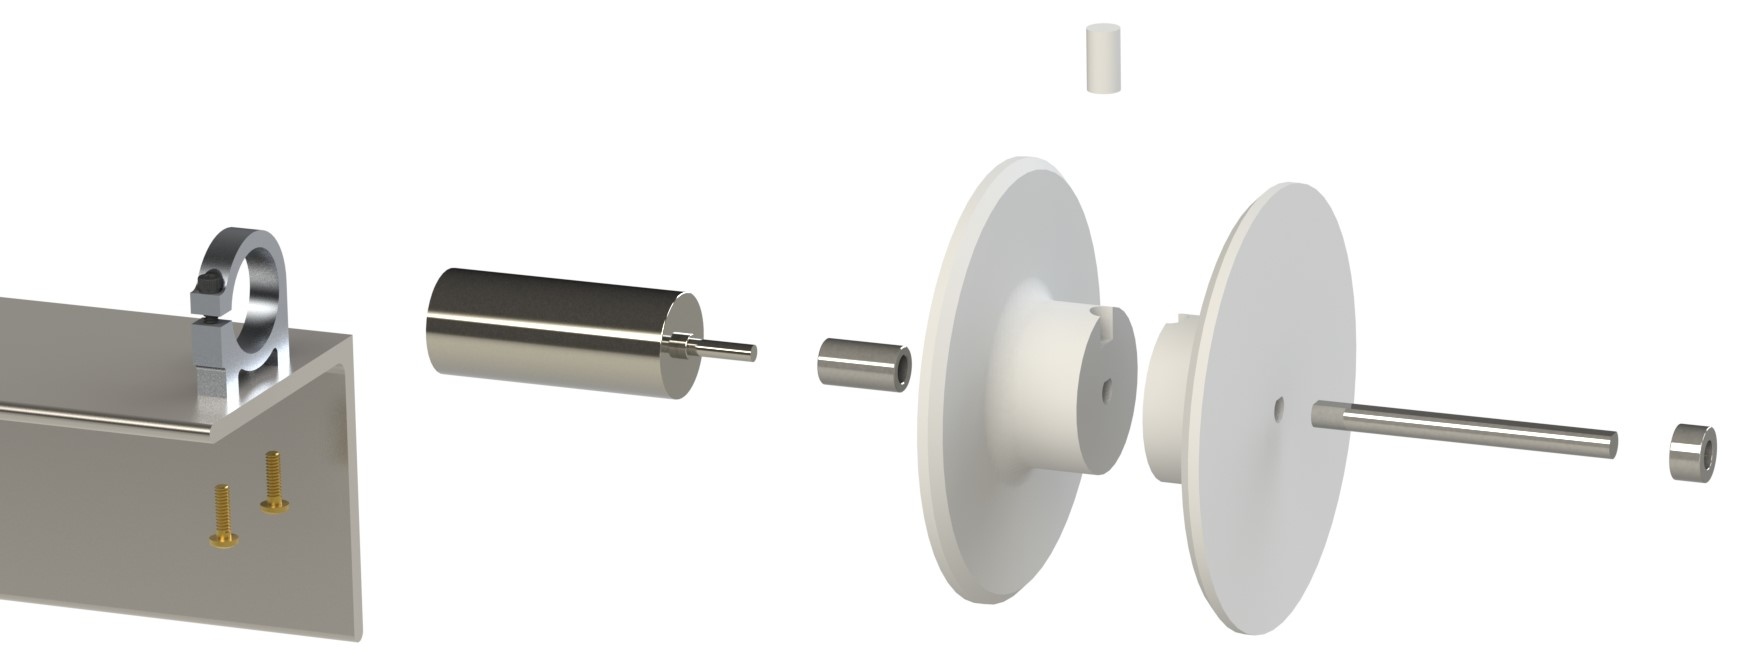
\includegraphics[width=0.9\textwidth]{./figs/qd_exploded.jpg}
	\caption{Solidworks Exploded View}
	\label{fig:qd_exploded}
\end{figure}

\begin{figure}[h!]
	\centering
	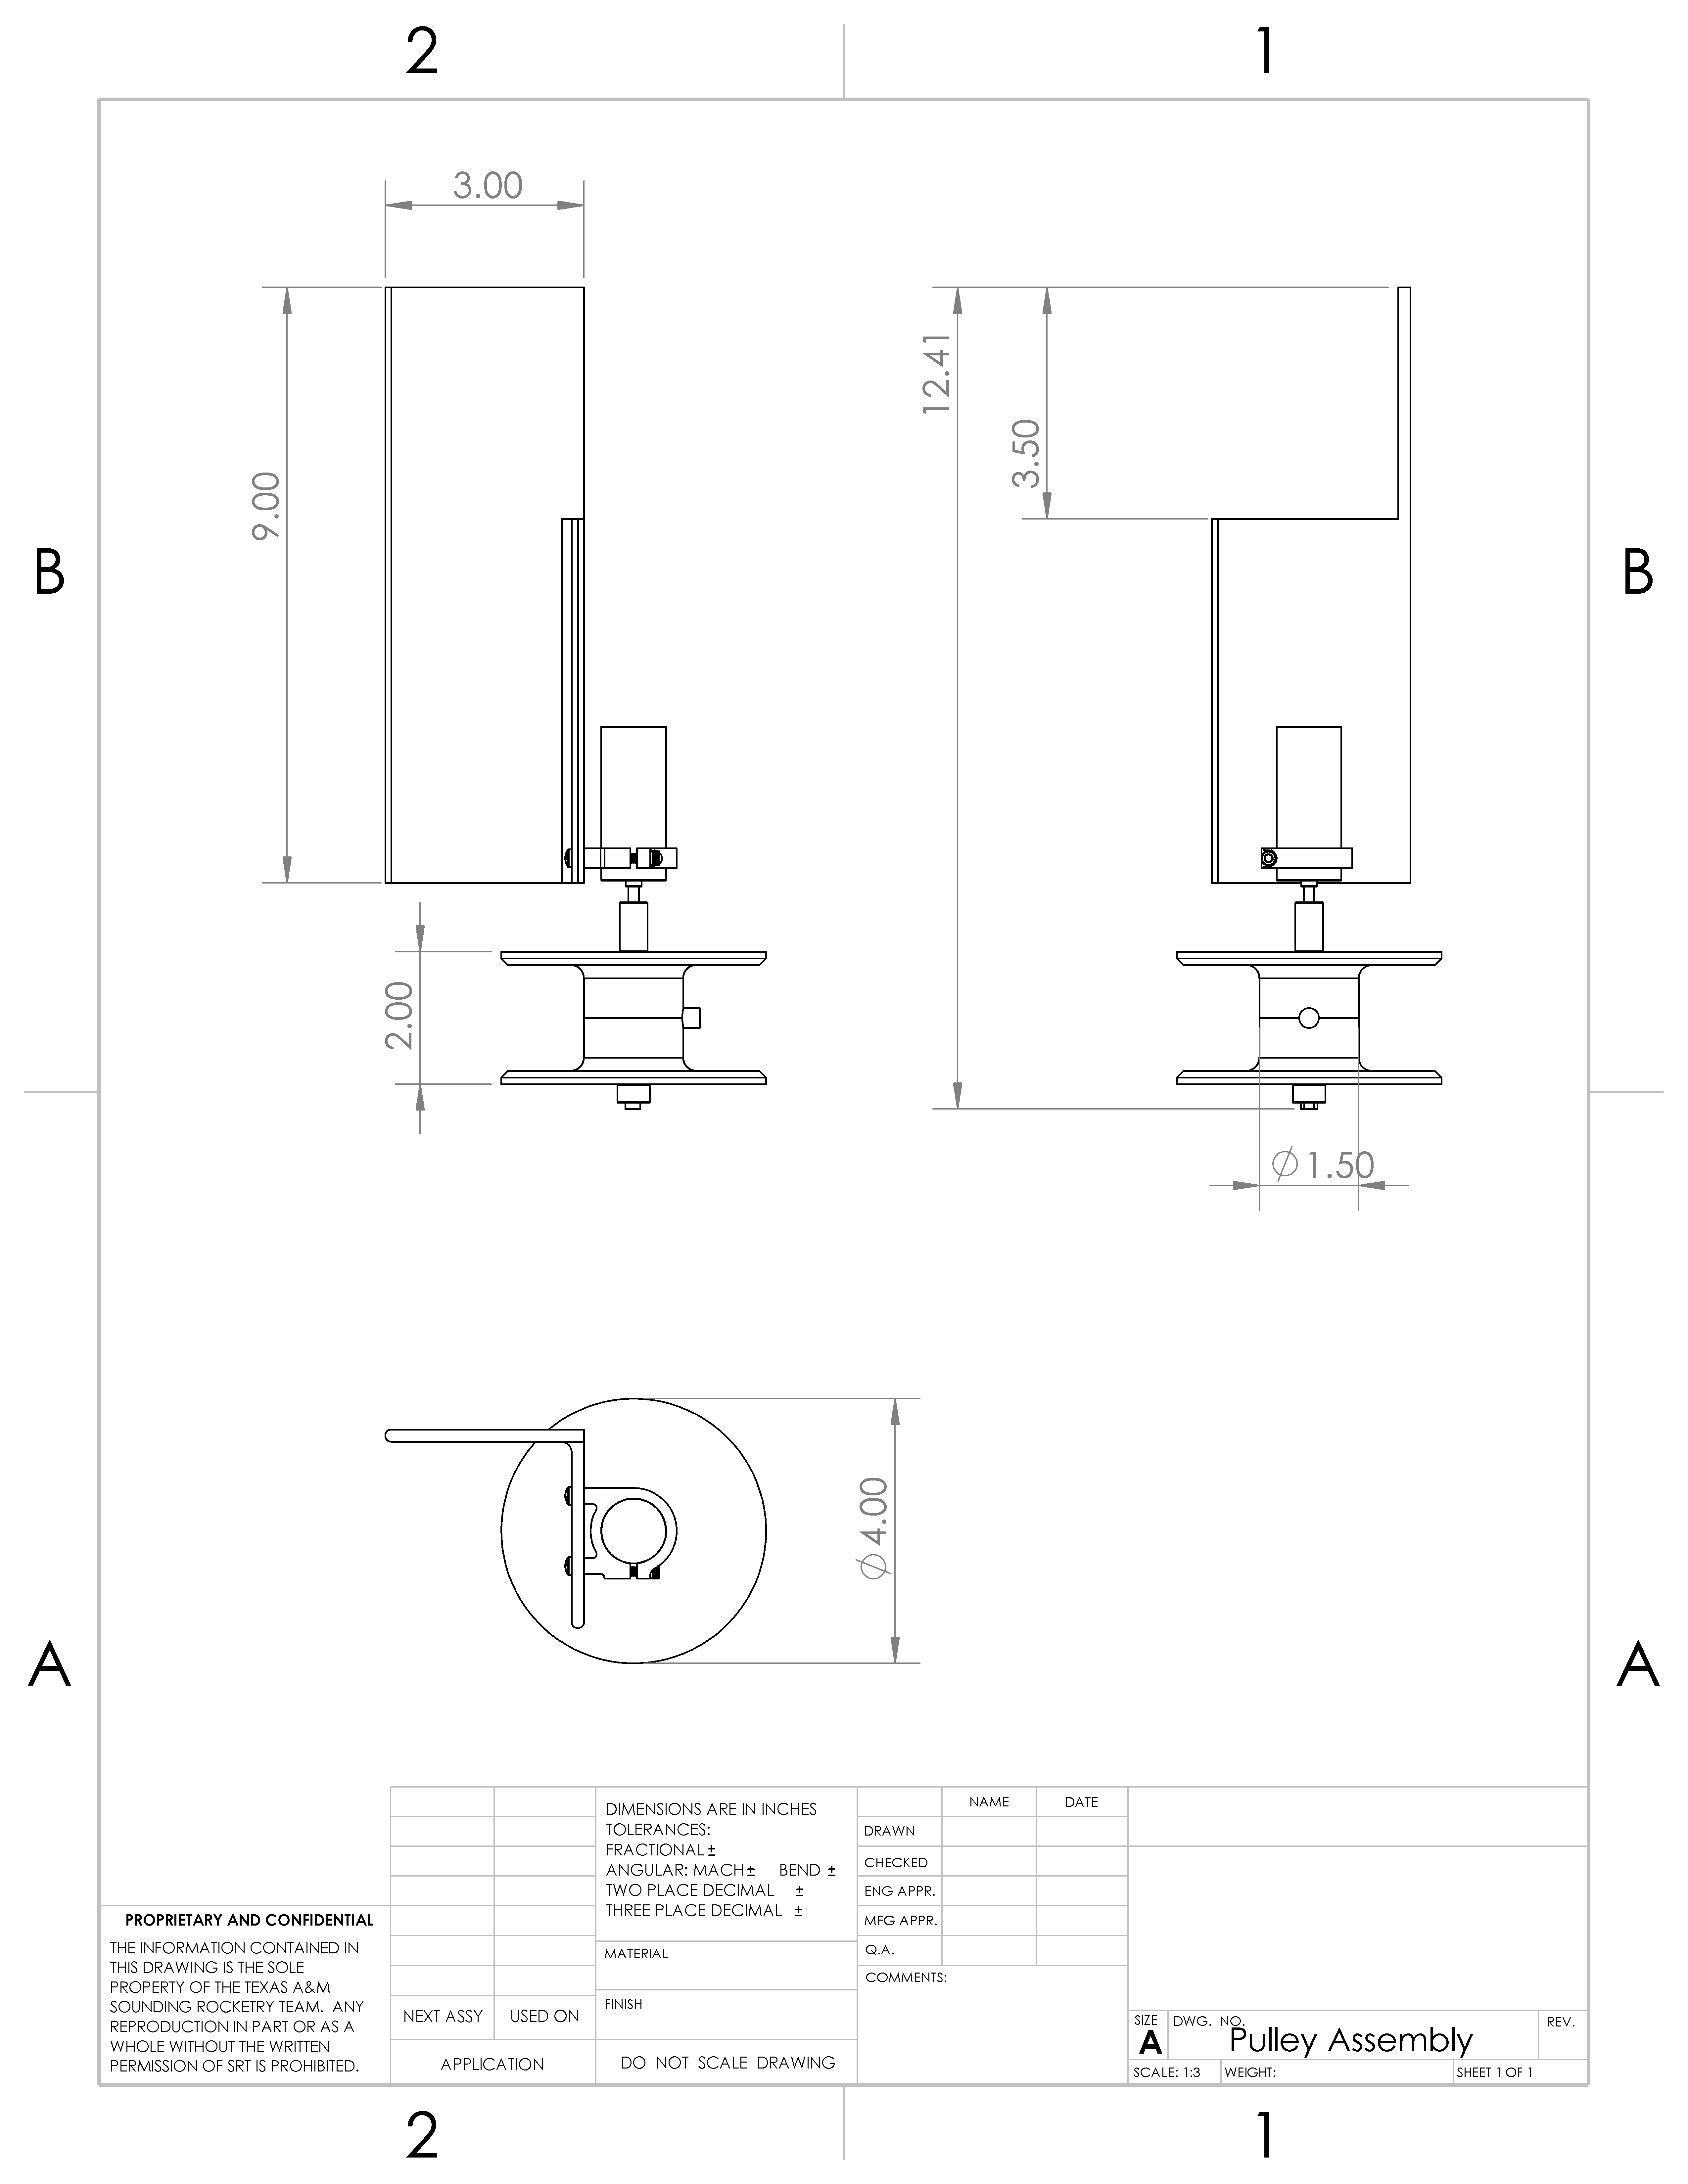
\includegraphics[width=1.0\textwidth]{./figs/qd_draw.png}
	\caption{Solidworks Drawing with Dimensions}
	\label{fig:qd_draw}
\end{figure}

\newpage
\subsection{Manufacturing}

\subsubsection{3D Printing}
The pulley was separated into three parts for ease of printing. Two half pulleys and a peg were printed using ABS plastic with an infill of 15\%. The prototype pulley was not printed with tolerance in it's shaft hole and a mallet was required to properly mount the halves onto the D-shaft. However, this lack of tolerance allowed for an extremely tight fit and epoxy was not required to keep the parts together. This should be taken into consideration for future prints.
\subsubsection{Mounting system}
The Mounting system for the test cell was made using a 9 in long segment of 3 in angle iron with a thickness of 3/16 in. The cut out section of the angle iron was cut using a band saw then ground flat with an angle grinder. Two holes for the motor clamp were made using a drill press. The completed assembly can be seen in figure  \ref{fig:qd_completed}.

\begin{figure}[h!]
	\centering
	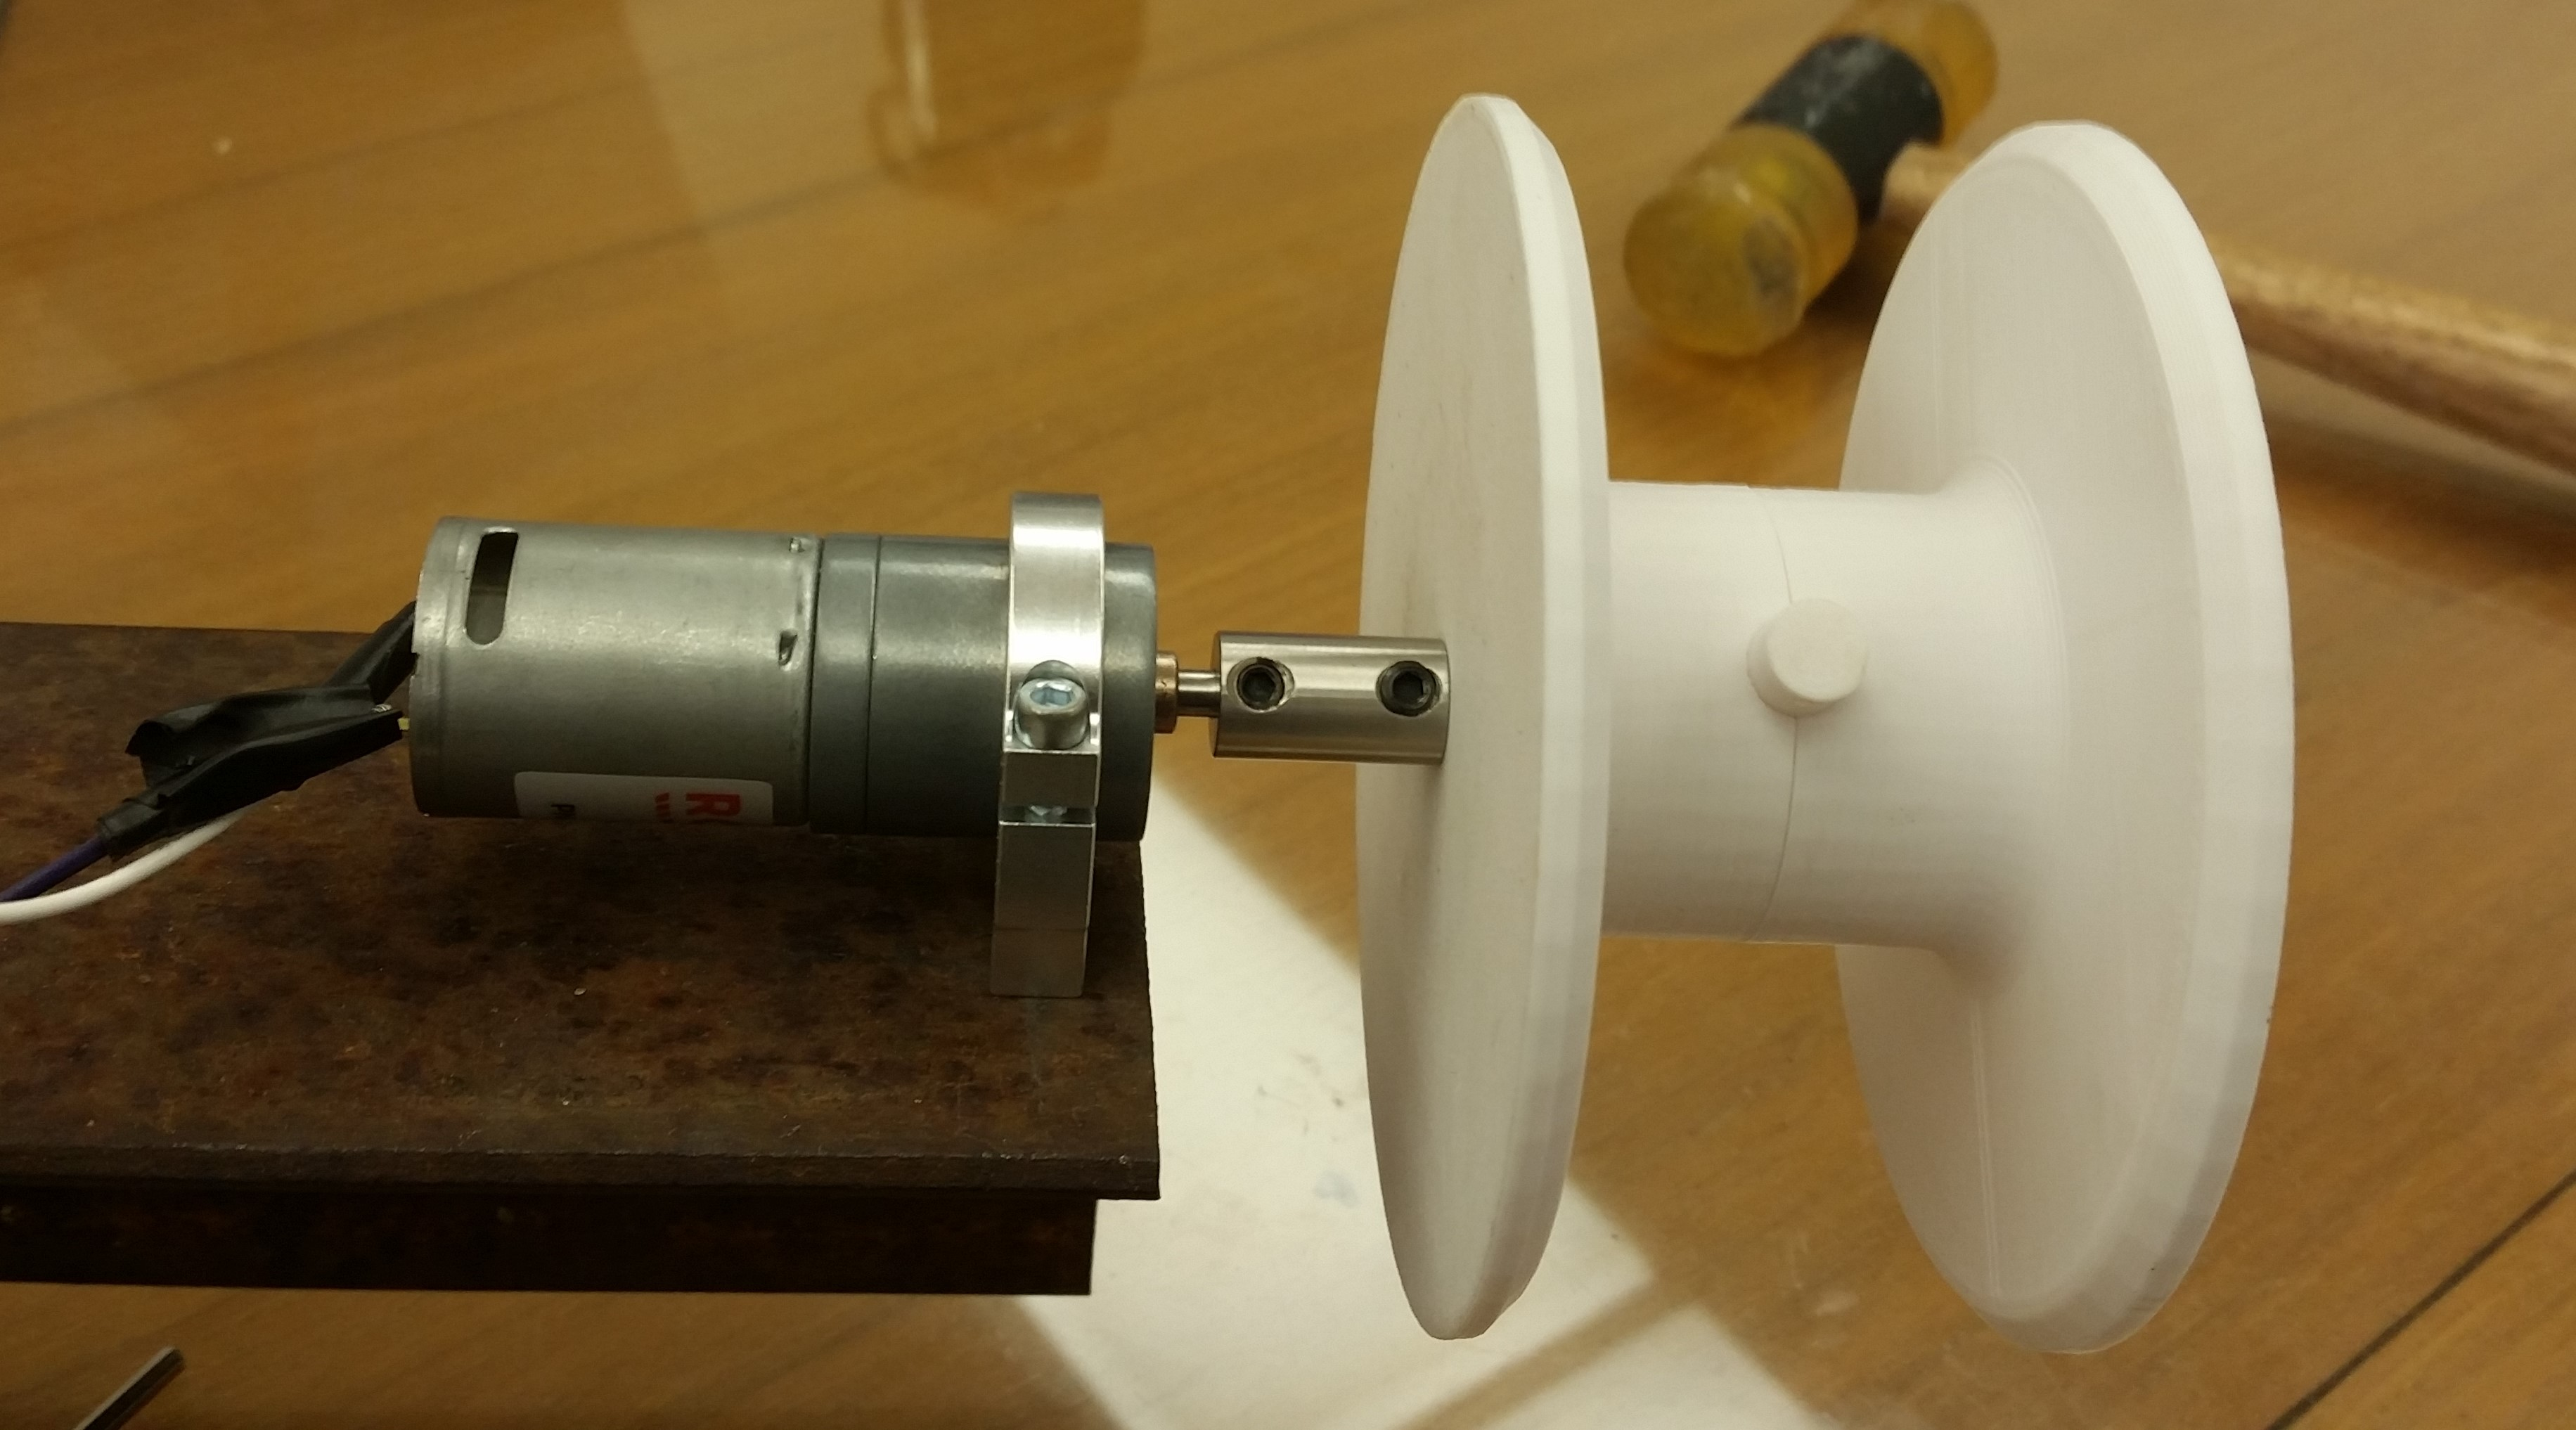
\includegraphics[width=.9\textwidth]{./figs/qd_completed.jpg}
	\caption{Completed Pulley Assembly}
	\label{fig:qd_completed}
\end{figure}

\subsection{Testing}

Two tests were done with the completed prototype mounted to the test cell. The Quick disconnect was attached with high strength fishing line to the pulley and the 12v battery was manually connected to initiate the disconnect. The first test performed as desired and the quick disconnect popped apart. During the second test the quick disconnect became stuck and the motor stalled. The stall damaged the gear train in the motors gearbox rendering it useless. Despite the motor breaking a lot of valuable information was gained. The 3D printed parts held up under full torque and the pulley was able to transfer the force necessary to disconnect the fill line. In other words, the design works fundamentally; All that is required is either a more resilient motor or a system to reduce risk of motor stall.

\begin{figure}[h!]
	\centering
	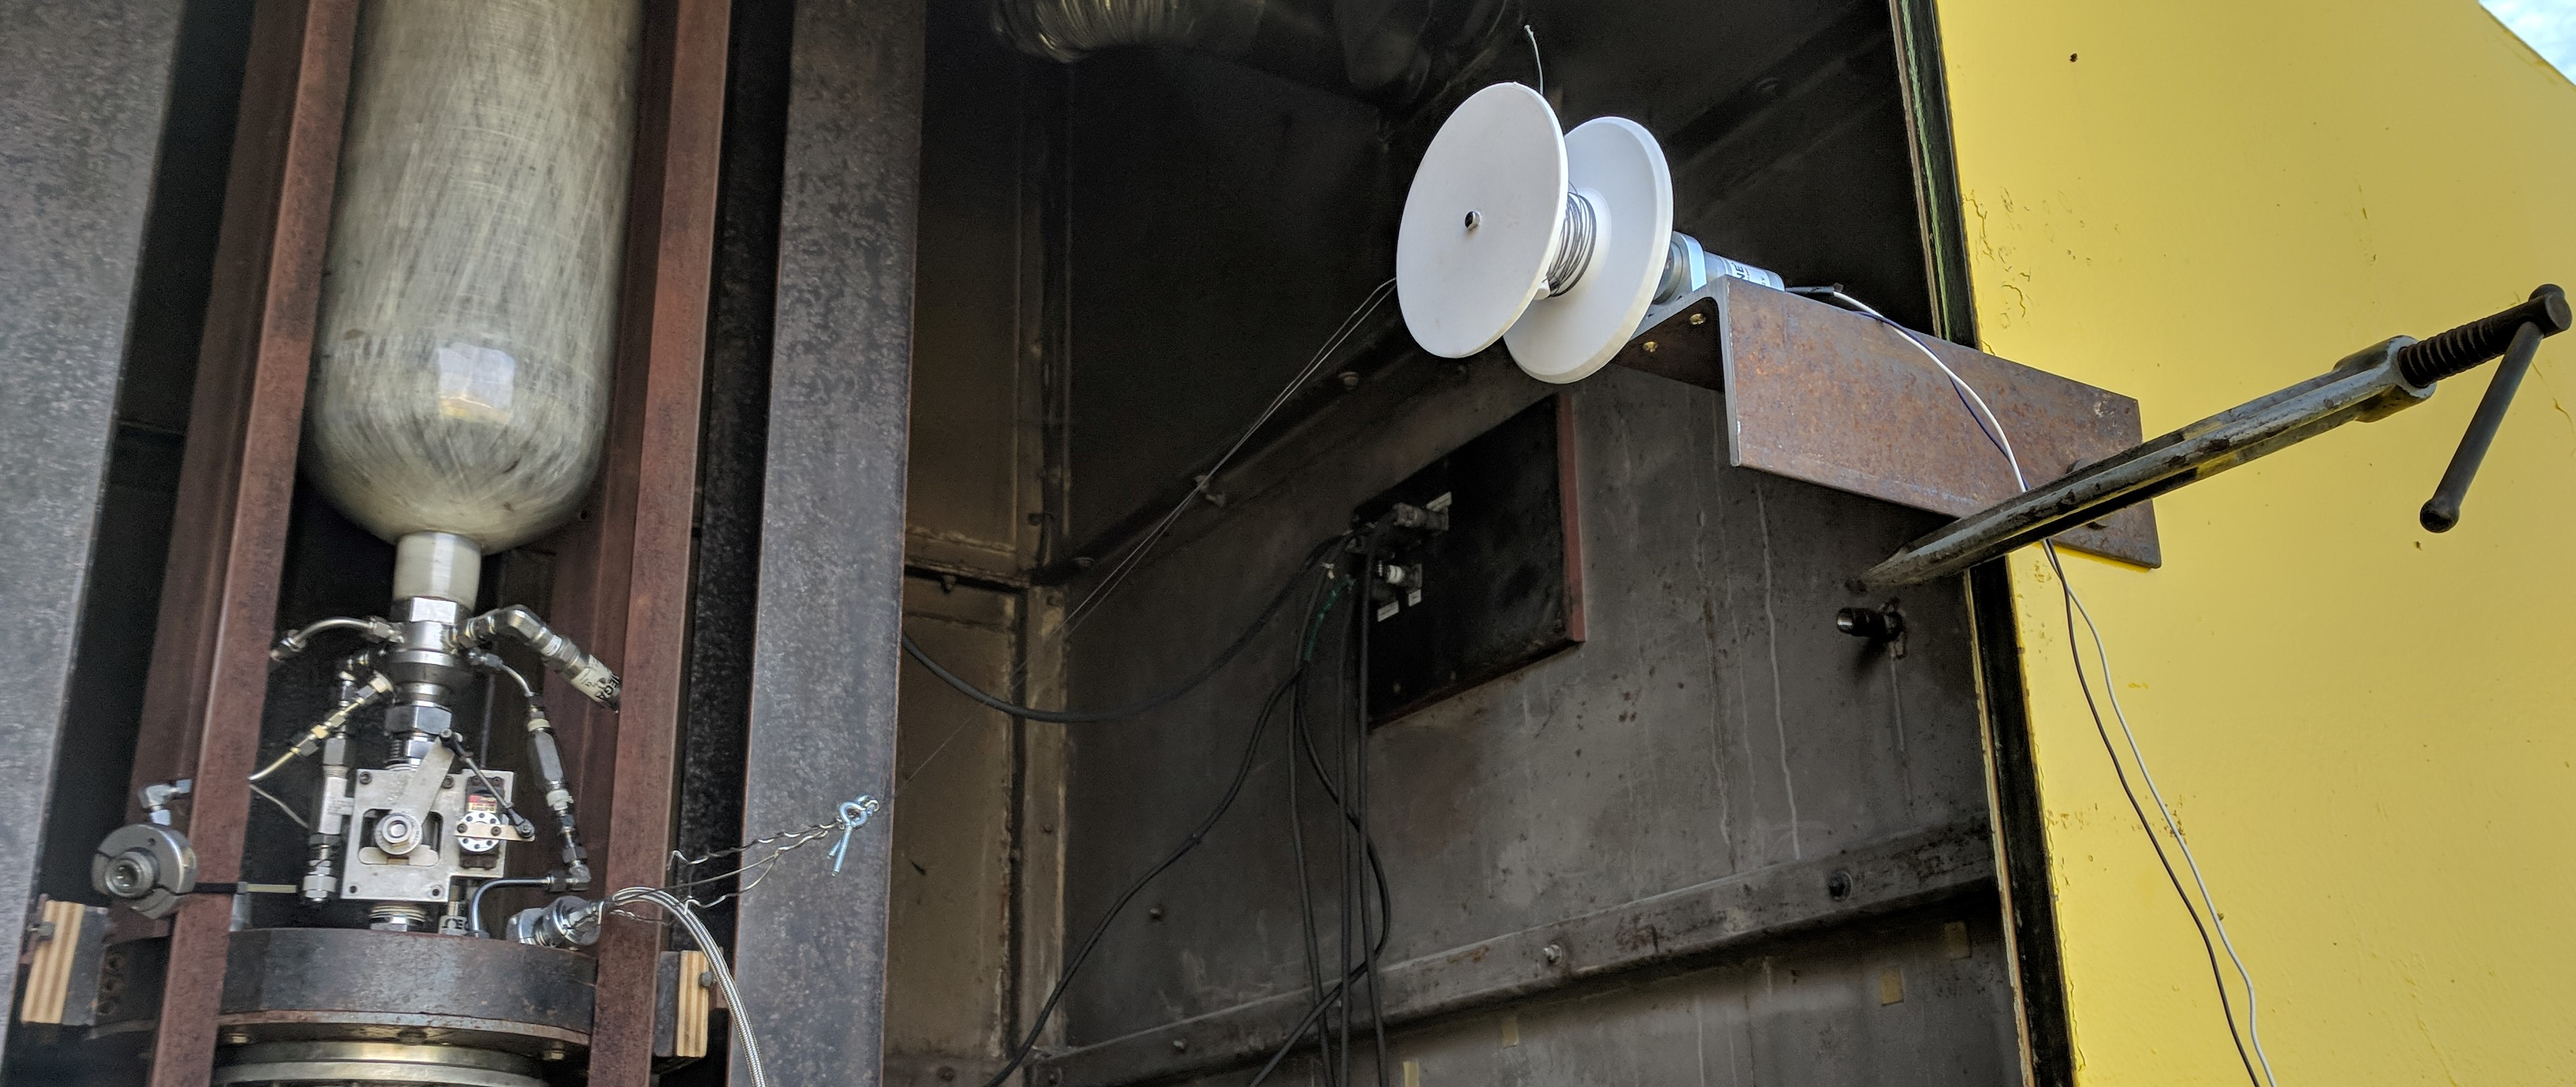
\includegraphics[width=1.0\textwidth]{./figs/qd_setup.jpg}
	\caption{Pulley Assembly in Test Configuration}
	\label{fig:qd_setup}
\end{figure}

\begin{figure}[h!]
	\centering
	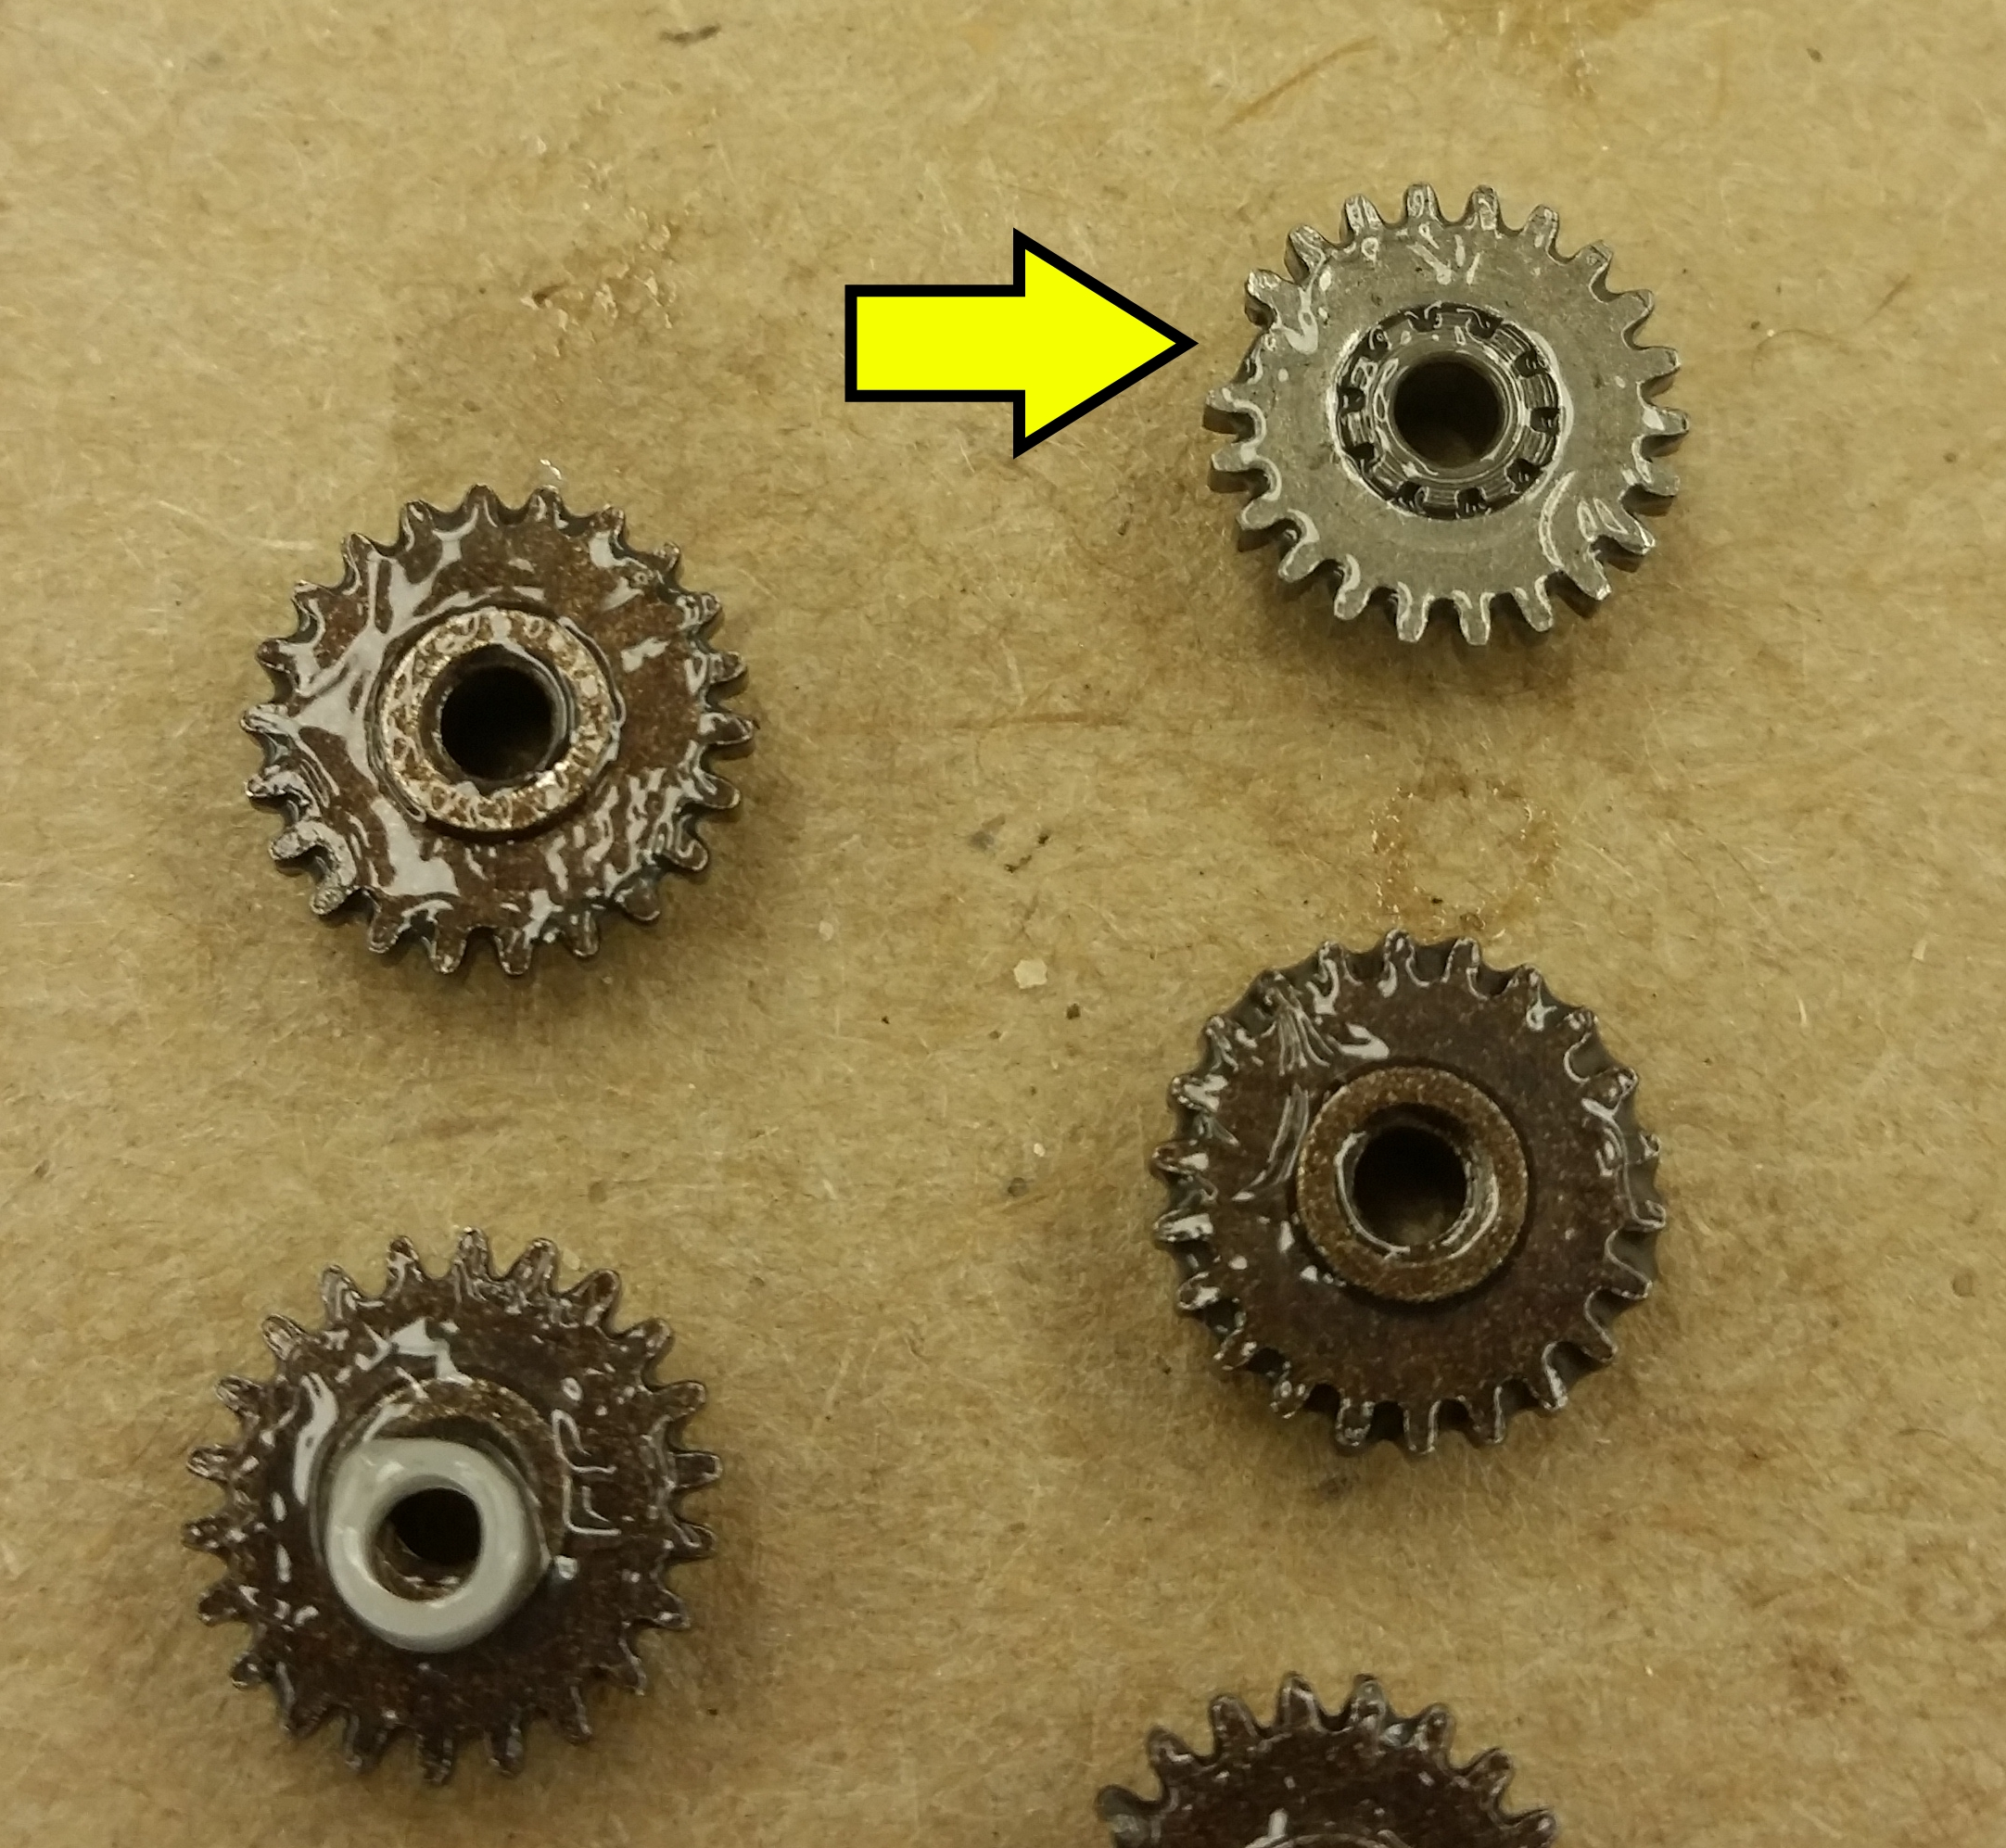
\includegraphics[width=.5\textwidth]{./figs/qd_gear.jpg}
	\caption{Damage to the Motor's Gear}
	\label{fig:qd_gear}
\end{figure}


\end{document}